\documentclass[12pt]{article}
\usepackage{lscape, xcolor}
\usepackage{verbatim}
\usepackage{amsmath,amsthm,amssymb}
\usepackage{colonequals,color,multirow}
\usepackage{enumerate}
\usepackage[sc]{mathpazo} % Use the Palatino font
\usepackage[T1]{fontenc} % Use 8-bit encoding that has 256 glyphs
\usepackage{times}	
% \usepackage{apacite}
\usepackage[authoryear]{natbib}
\usepackage[demo]{graphicx}
\usepackage{subcaption}
\usepackage{lscape, xcolor}
\usepackage{verbatim}
\usepackage{amsmath,amsthm,amssymb}
\usepackage[sc]{mathpazo} % Use the Palatino font
\usepackage[T1]{fontenc} % Use 8-bit encoding that has 256 glyphs
\usepackage{times}	
\usepackage{booktabs}
\usepackage{ caption, float}
\usepackage{enumitem}
\usepackage[left=1in, right=1in, top=1in, bottom=1in]{geometry}
\usepackage{blindtext}
\usepackage{titlesec}
\usepackage{array}
\usepackage{graphicx}
%\graphicspath{/home/evo/4m_final_project}
\setcounter{secnumdepth}{4}
\usepackage{caption} % For subfigures with captions
\usepackage{subcaption} % For subfigures with captions
\captionsetup[subfigure]{labelformat=empty} % Removes the (a), (b) labels
\usepackage{hyperref}
\usepackage[authoryear]{natbib}
\titleformat{\paragraph}
{\normalfont\normalsize\bfseries}{\theparagraph}{1em}{}
\titlespacing*{\paragraph}
{0pt}{3.25ex plus 1ex minus .2ex}{1.5ex plus .2ex}
\renewcommand{\baselinestretch}{1.5}% Line spacing - Palatino needs more space 
\vspace{\baselineskip}
\linespread{1.5}




\begin{document}

\title{STATS 4M03: Multivariate Analysis\\ Final Project \\ Diabetes Dataset }

\author{Submitted to\\ Dr. Eman M.S. Alamer 
\\Department of Mathematics and Statistics
\\McMaster University\\Hamiltion, Ontario, Canada L8S 4K1}
\date {November 22, 2024}


\maketitle

 \centerline{Reported by}
 \centerline{Xinyi Chen (400326045)}
  \centerline{Tonu Xu(400370837)}
   \centerline{Rayyan Kazim(Student ID)}
    \centerline{Safi Khan (400402095)}
     \centerline{First last (Student ID)}


\newpage
%\thispagestyle{fancy} % All pages have headers and footers
\section{Introduction}
\subsection{Abstract}

The study of diabetes is vital in understanding the progression of the disease and identifying key predictors. Throughout this paper, we perform data analysis on the diabetes dataset, primarily focusing on leveraging various statistical methods that we learned in STATS 4M03$\backslash$6M03: Multivariate Analysis. By using a variety of methods, our goal is to predict the onset of diabetes from detailed medical diagnostic measurements based on several contributing health factors --- with the aim of uncovering patterns and relationships between various clinical and lifestyle factors. Through this analysis, we hope to emphasize actionable insights for clinical decision-making and provide preventive strategies. 

\subsection{The Data}

In this paper, we will study the diabetes dataset. \cite{Kaggles} which can be found here: \href{https://www.kaggle.com/datasets/hasibur013/diabetes-dataset}{Diabetes Dataset}. The diabetes dataset contains 768 rows x 9 columns, representing various health diagnostic metrics for predicting diabetes. Each row corresponds to a unique patient record, with features capturing key medical attributes. Table~\ref{tab:DibetesTab} showcases each of the columns in the dataset and a description of each of the columns. We will be using R \cite{Rlang} as our main computing software

\begin{table}[h!]
	\centering
	\resizebox{\textwidth}{!}{ % Resize to fit the width of the page
	\begin{tabular}{|c|c|}
		\hline
		\textbf{Column} & \textbf{Description Of Column} \\ \hline
		Pregnancies & Integer: Number of times the patient has been pregnant. \\ \hline
		Glucose & Integer: Plasma glucose concentration (mg/dL) after a 2-hour oral glucose tolerance test. \\ \hline
		BloodPressure & Integer: Diastolic blood pressure (mm Hg). \\ \hline
		SkinThickness & Integer: Triceps skinfold thickness (mm). \\ \hline
		Insulin & Integer: 2-hour serum insulin (mu U/ml). \\ \hline
		BMI  & Float: Body mass index, defined as weight in kg/(height in m)\^2. \\ \hline
		DiabetesPedigreeFunction & Float: A score indicating genetic predisposition to diabetes based on family history. \\ \hline
		Age & Integer: Age of the patient (in years). \\ \hline
		Outcome & Binary: Target variable where 1 indicates diabetes, and 0 indicates no diabetes. \\ \hline
	\end{tabular}
}
	\caption{Description of the Diabetes Dataset}
	\label{tab:DibetesTab}
\end{table}

\subsubsection{Exploratory Data Analysis (EDA)}

\begin{enumerate} 
	
	\item The diabetes dataset consists of 768 observations and 9 variables. All variables are integers, except for "BMI" and "DiabetesPedigreeFunction", which are labelled as numeric. This dataset does not consist of any N/A values or duplicated rows. 
	
	\item A summary statistics table was used to show the mean, median, minimum and maximum values of each variable, as well as quartiles. There are a lot more observations without diabetes than with diabetes. The ages listed in this dataset follow a right-skewed distribution, where majority of the individuals are aged 20-30. 
	
	\item "SkinThickness" is well correlated with "BMI" and "Insulin". "Glucose" is reasonably correlated with "Insulin", "BMI" and also "Age". "Age" is well correlated with "Pregnancies". 
	
	\item The dataset will be split into 2, where 1 will be the response variable, "Outcome". The other will consist of all the other variables, which are considered the predictor variables. All predictors should be used as they all are numeric/integer variables who are well/reasonably correlated with each other. 75 percent of the data will be used for training, whereas the rest will be used for testing. 
	
	\item For dimensionality reduction, we cannot use factor analysis since the dataset is not normally distributed. This can be confirmed by the shapiro test and normal QQ plot. For dimensionality reduction, we would use principal component analysis. We will use 3 principal components.\\  
	
	
	
	\begin{figure}[h!] 
		
		\centering 
		
		\fbox{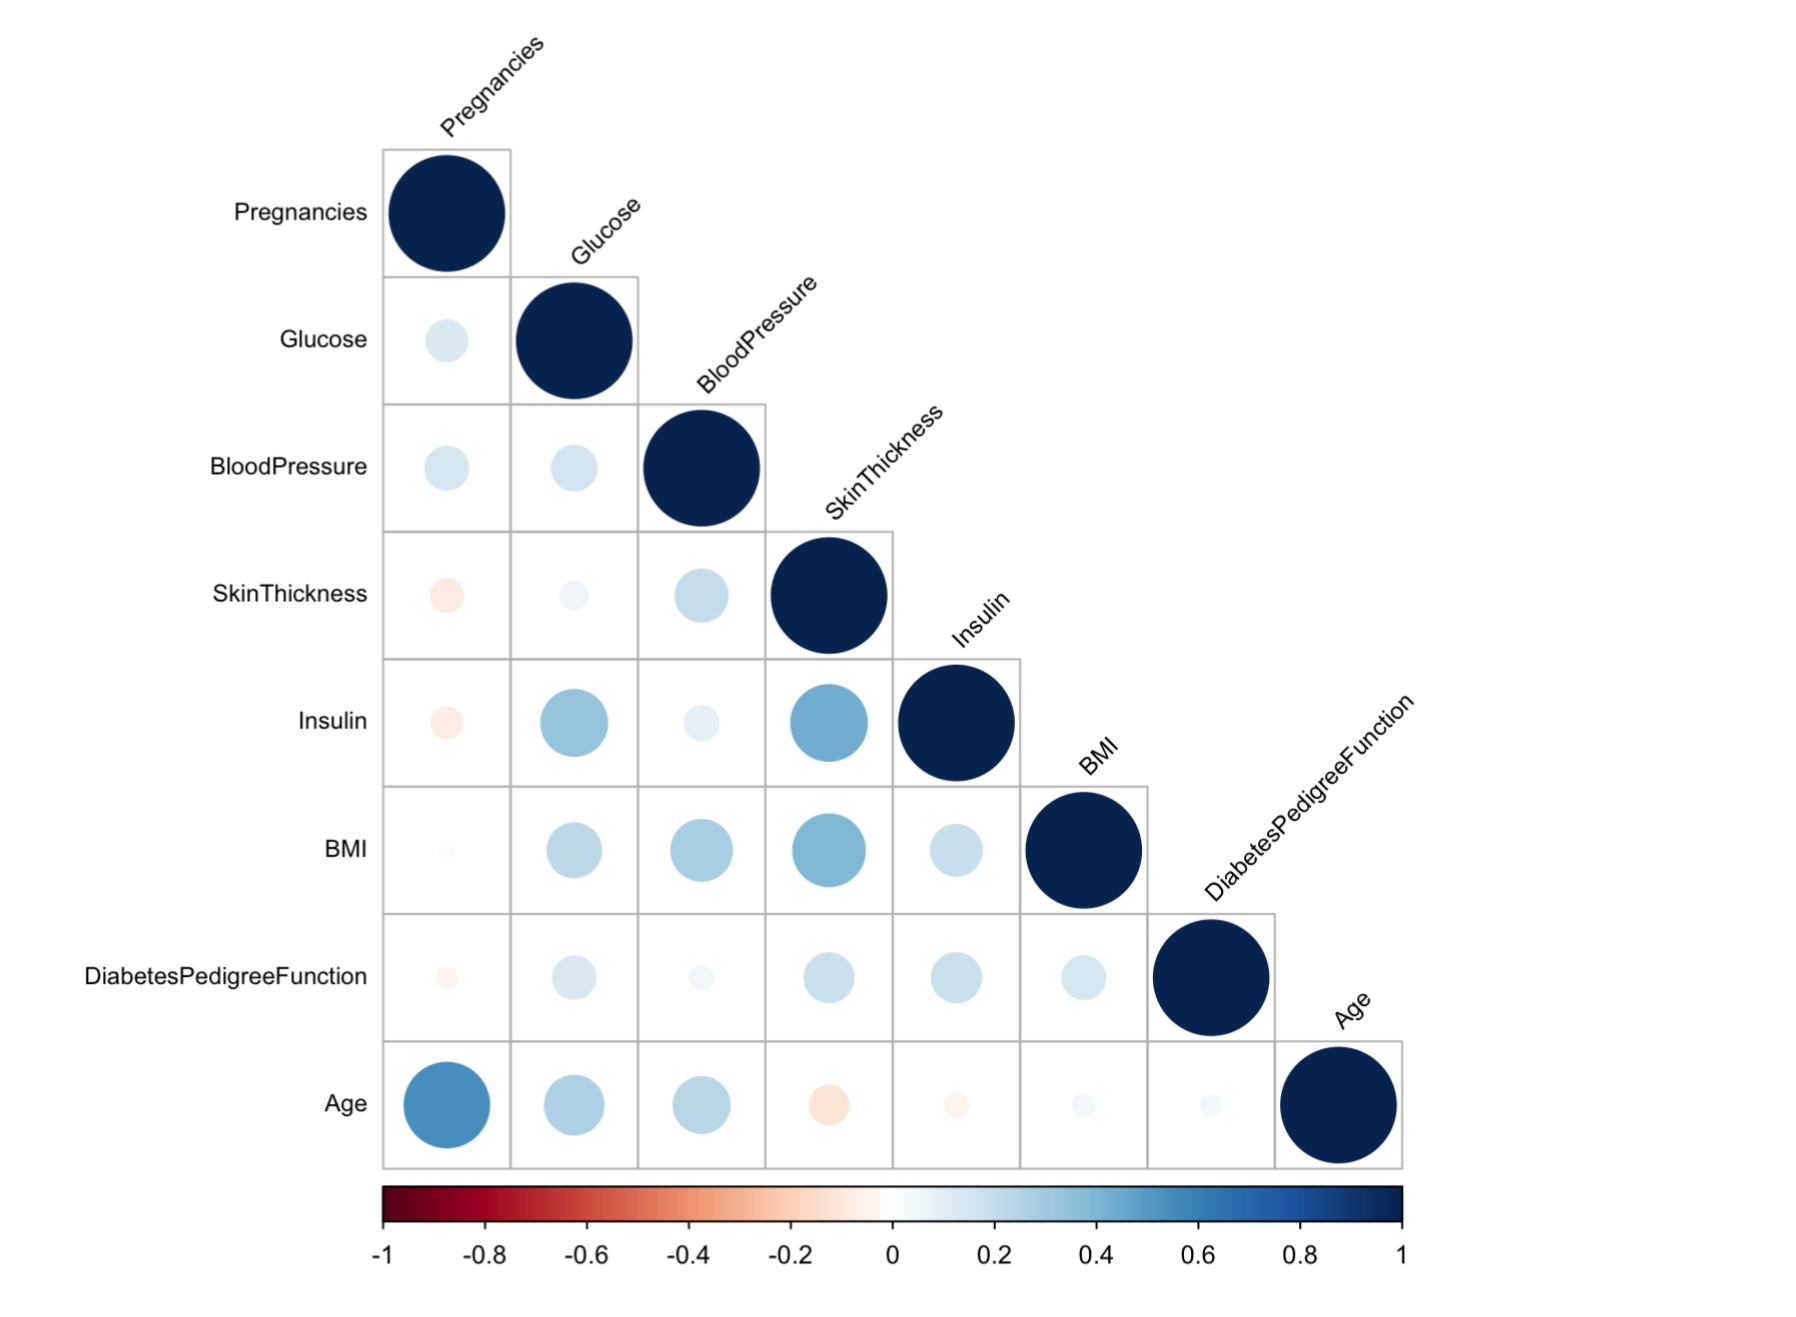
\includegraphics[width=0.62\textwidth]{correlations2.png}} 
		
		\caption{Correlation Plot} 
		
		\label{fig:corplot} 
		
	\end{figure} 
	
	
	
	\begin{figure}[h!] 
		
		\centering 
		
		\fbox{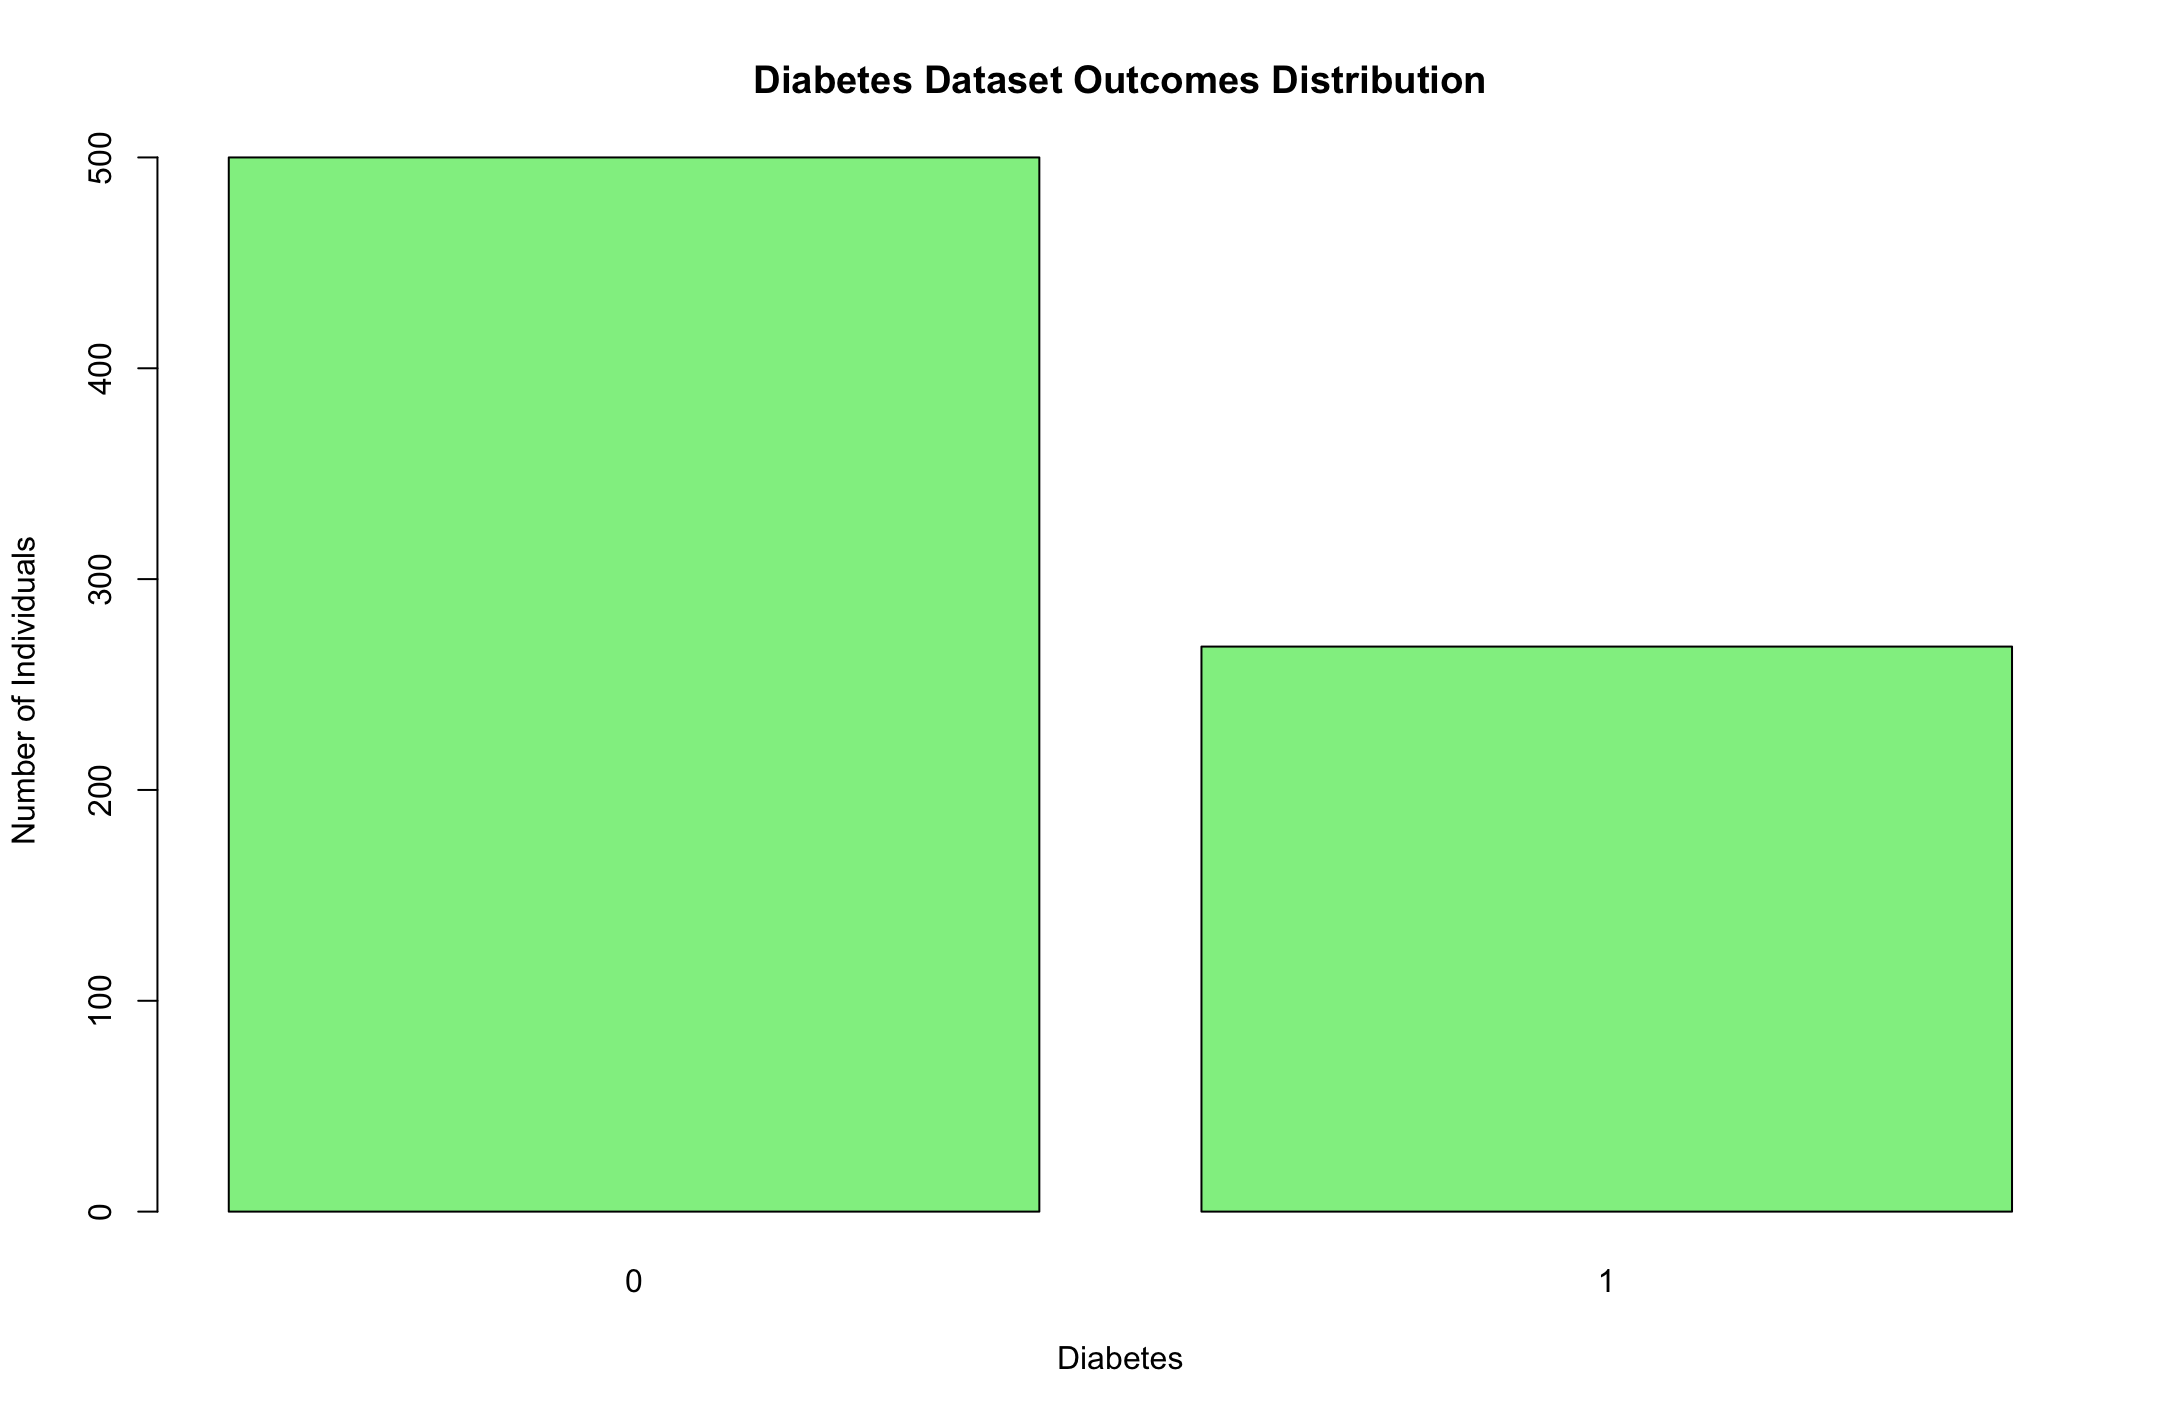
\includegraphics[width=0.62\textwidth]{outcomes.png}} 
		
		\caption{Outcomes Plot} 
		
		\label{fig:barplot} 
		
	\end{figure} 
	
	
	
	\begin{figure}[h!] 
		
		\centering 
		
		\fbox{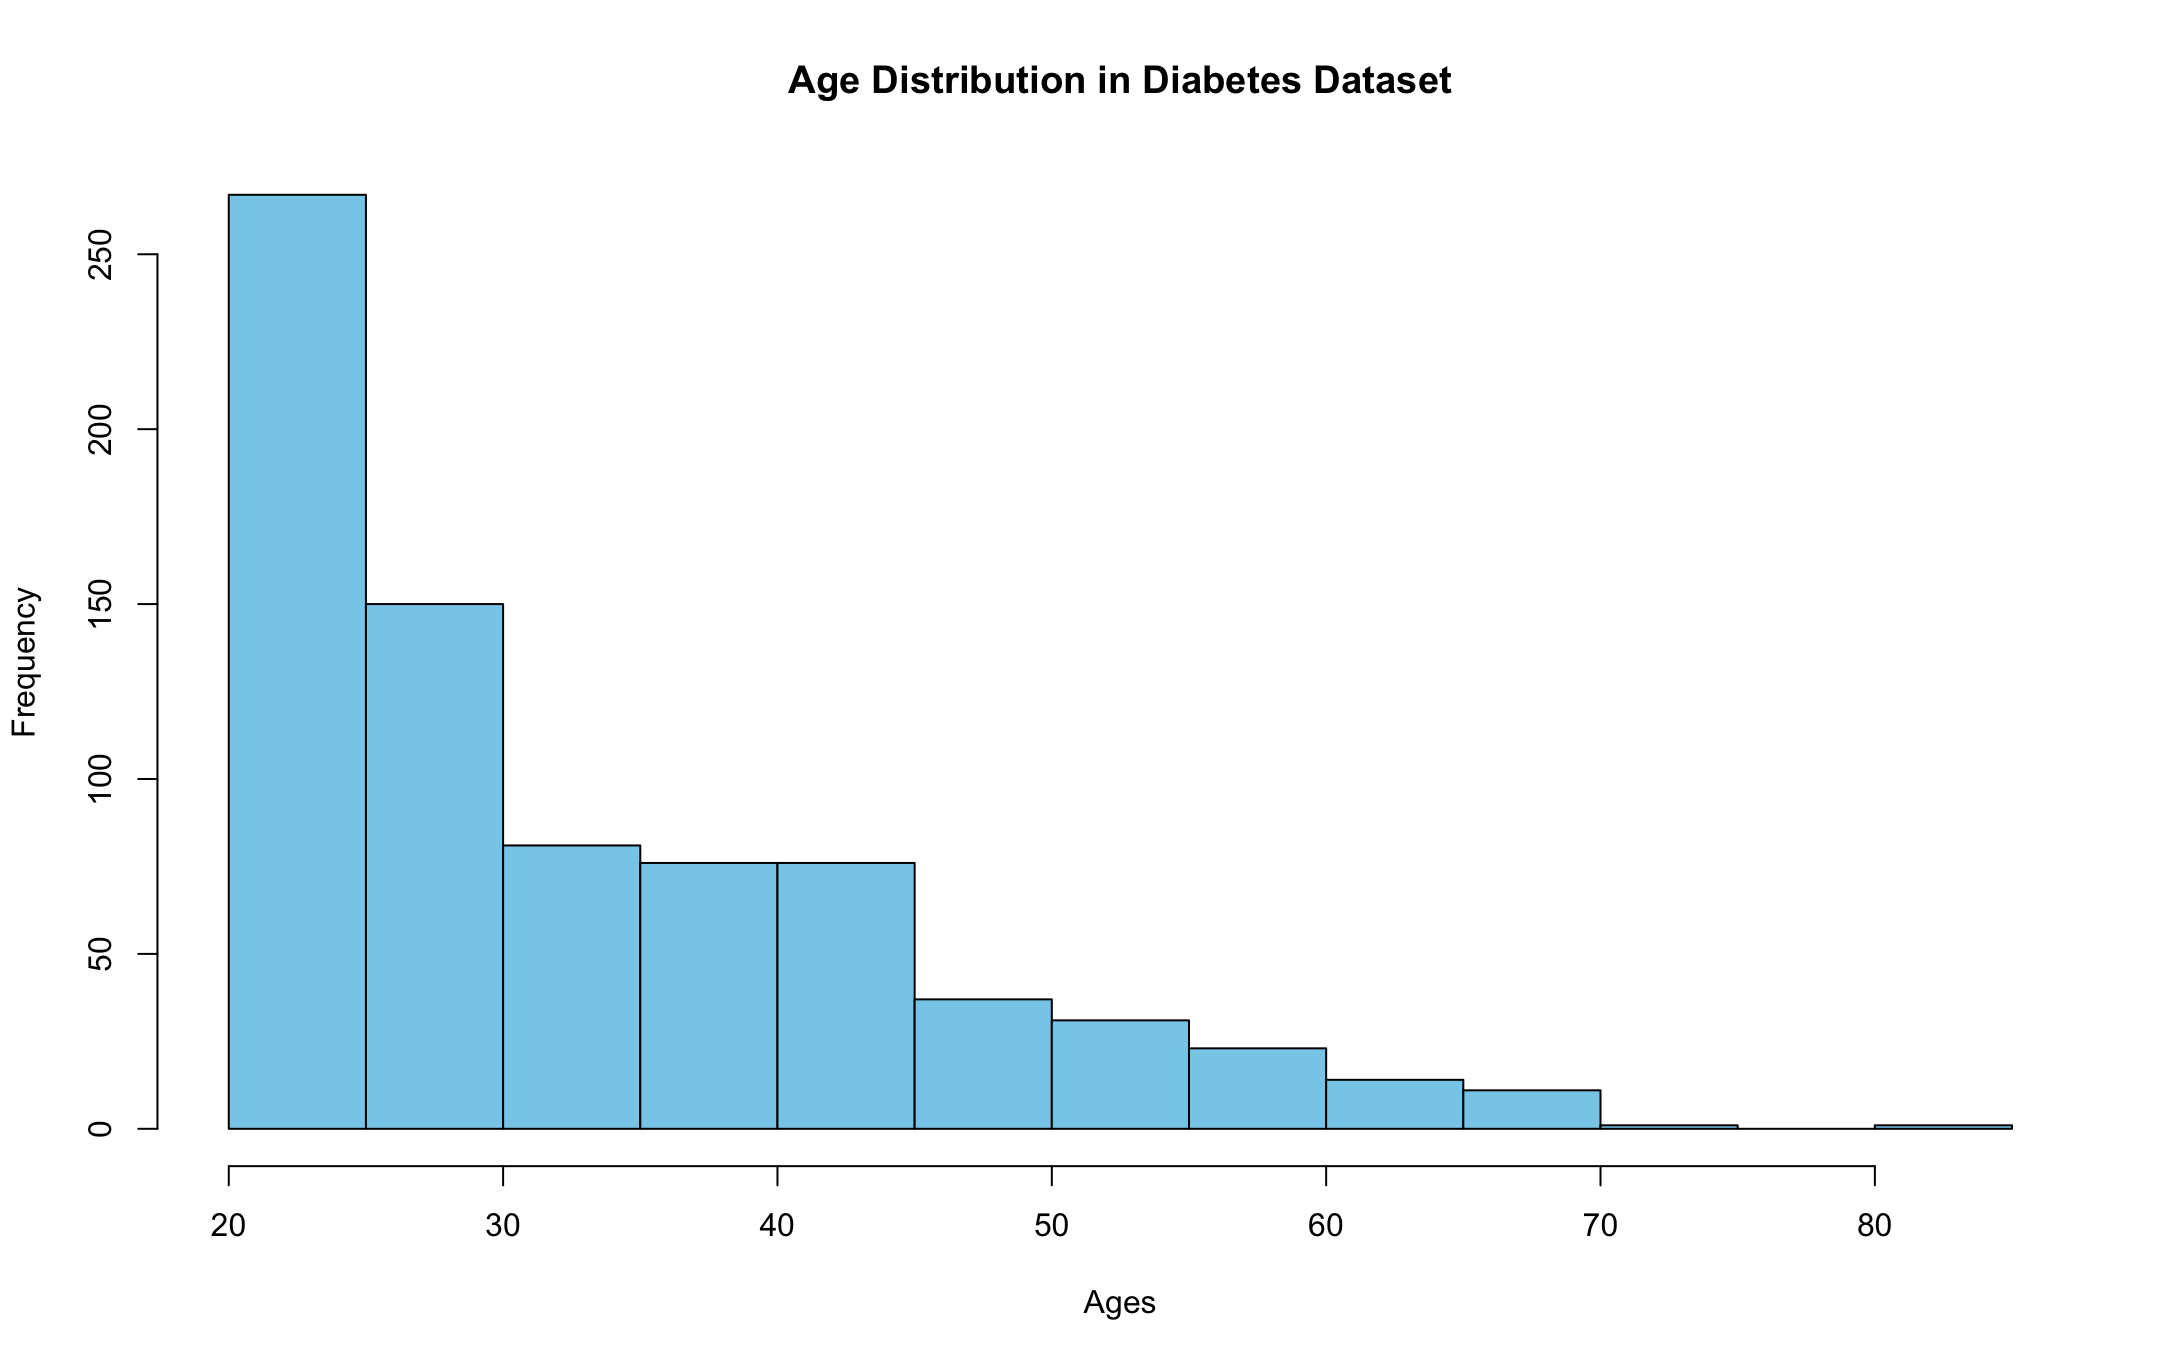
\includegraphics[width=0.62\textwidth]{ages.png}} 
		
		\caption{Ages Plot} 
		
		\label{fig:histplot} 
		
	\end{figure} 
	
	
	
	\begin{figure}[h!] 
		
		\centering 
		
		\fbox{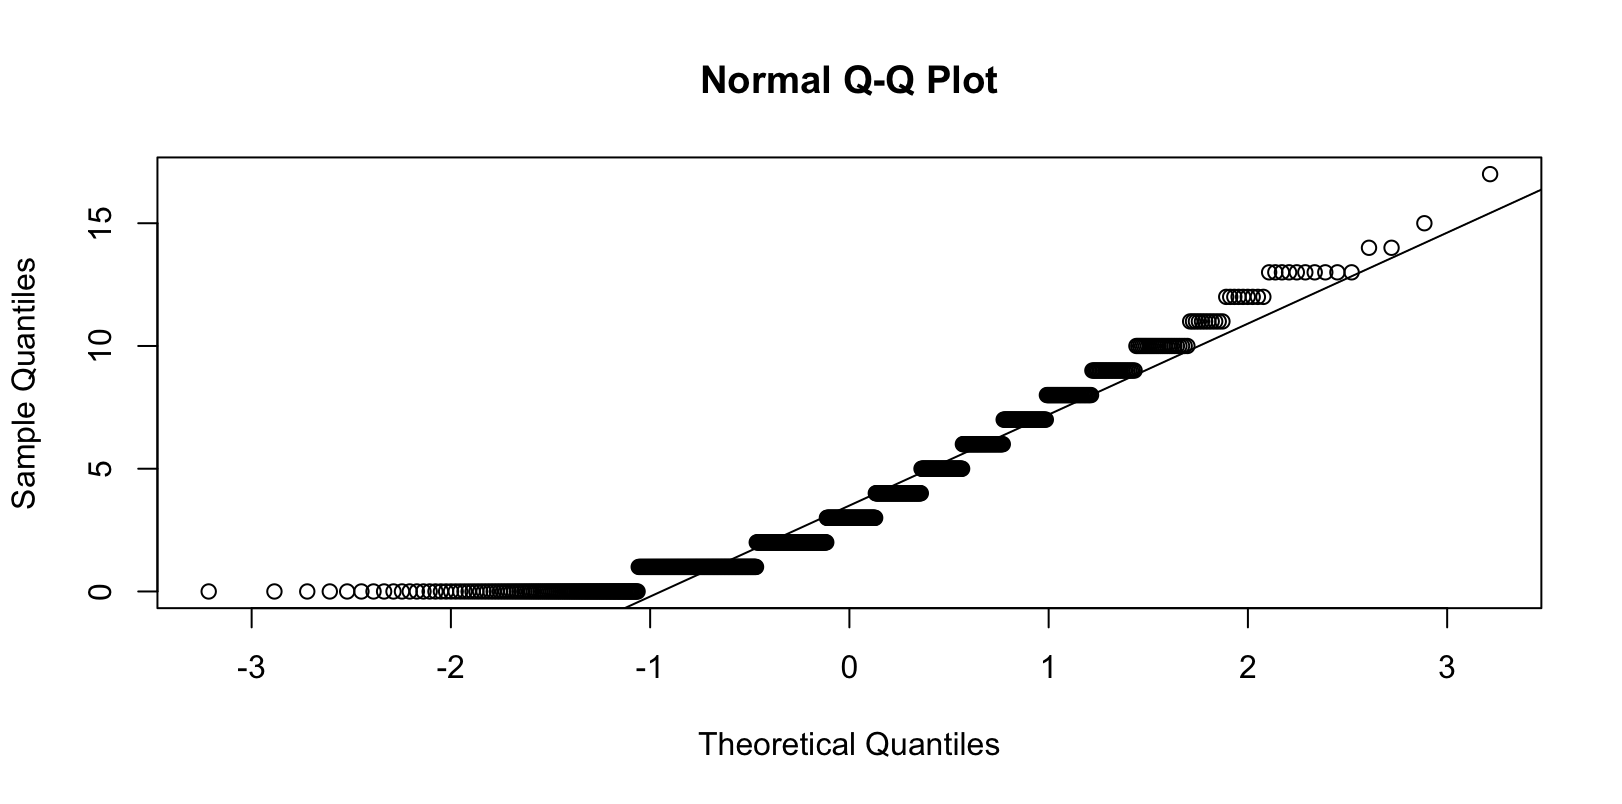
\includegraphics[width=0.62\textwidth]{normal.png}} 
		
		\caption{Normality Checking Plot} 
		
		\label{fig:normalplot} 
		
	\end{figure} 
		
\end{enumerate} 
 

\subsubsection{Data Preparation} 

We write about the training and testing here, and how we used column 9 as a label. We also scaled the dataset.\\

\section{Methodology}
\subsection{Supervised learning Analysis} 
 In this section, we perform supervised learning analysis using Classification trees: k-Nearest Neighbours and the following ensembles method: Random Forests Classifiers.\cite{zhou2012ensemble}
 
 \subsubsection{k-Nearest Neighbours}

 Firstly, we executed the k-Nearest Neighbours algorithm \cite{peterson2009k} on our dataset. The algorithm is a non-parametric, supervised learning classifier that uses proximity to make classifications about the grouping of a dataset.

 \subsubsection{Random Forest Classifiers}
 
 Also, we used the Random Forest Classifiers \cite{zhou2012ensemble} on our dataset. Random Forest classifiers is a bootstrapping sampling method that combines the results of multiple decision trees to draw on a conclusion. The algorithm \cite{Lecture16} is an extension of the bagging algorithm \cite{Lecture16} that creates uncorrelated decision trees, for each tree, a random sample of $\mathcal{M}$ is taken at each decision tree split.

\subsection{Binary Logistic Regression}
We performed a binary logistic regression analysis \cite{faraway2016extending}, a supervised learning method, to explore the relationship between various predictor variables and the binary response variable “Outcome,” indicating the presence or absence of diabetes. The initial model incorporated eight predictor variables: Pregnancies, Glucose, Blood Pressure, Skin Thickness, Insulin, BMI, Diabetes Pedigree Function, and Age. These variables were selected based on their potential relevance to diabetes risk, informed by existing domain knowledge.\\
\setlength{\parindent}{0pt}
The objective of the analysis was to identify the most significant predictors using the backward elimination method, a stepwise regression technique. This approach began with a model including all predictors, subsequently removing variables in sequence based on the highest p-value exceeding 0.05. This systematic elimination of statistically insignificant predictors not only enhances the model’s interpretability but also minimizes the risk of overfitting, ensuring that the final model retains only variables with significant contributions to predicting the outcome.

\subsection{Boosting}

Boosting \cite{chen2015xgboost} \cite{friedman2001greedy} is an ensemble learning technique that combines multiple weak learners, typically decision trees, to create a strong predictive model. For this analysis, we used XGBoost (Extreme Gradient Boosting), which is efficient and optimized for large datasets, to predict the presence of diabetes based on clinical measurements.

The model was trained on 70\% of the data, leaving 30\% for testing. The binary outcome variable (1 = diabetes, 0 = no diabetes) was predicted using features such as glucose levels, BMI, and age. Missing or zero values were present in some predictors (e.g., insulin), which could influence the model's performance.

\textbf{Model Parameters}
\begin{itemize}
	\item Learning rate (\texttt{eta}): 0.1
	\item Maximum tree depth (\texttt{max\_depth}): 6
	\item Evaluation metric: Area Under the Curve (AUC)
	\item Number of boosting rounds (\texttt{nrounds}): 100
\end{itemize}

\section{Discussion}
\subsection{Binary Logistic Regression}

\begin{table}[h!]
	\centering
	\resizebox{0.80\textwidth}{!}{%
	\begin{tabular}{|c|c|c|c|c|}
		\hline
		Coefficients & Estimate & Std. Error & Z-Value & Pr(>|Z|) \\ \hline
		(Intercept) & -8.4398695 & 0.8176393 & -10.322 & < 2e-16 \\ \hline
		Pregnancies & 0.1135092 & 0.0375672 & 3.021 & 0.00252 \\ \hline
		Glucose & 0.0343876 & 0.0042392 & 8.112 & 4.99E-16 \\ \hline
		BloodPressure & -0.0134342 & 0.0059047 & -2.275 & 0.0229 \\ \hline
		SkinThickness & 0.0098866 & 0.0083722 & 1.181 & 0.23765 \\ \hline
		Insulin & -0.0015283 & 0.0009882 & -1.546 & 0.122 \\ \hline
		BMI & 0.0776662 & 0.0174657 & 4.447 & 8.72E-06 \\ \hline
		DiabetesPedigreeFunction & 0.8088779 & 0.332009 & 2.436 & 0.01484 \\ \hline
		Age & 0.0297298 & 0.0109345 & 2.719 & 0.00655 \\ \hline
	\end{tabular}%
}
	\caption{Binary Logistic Regression Output}
	\label{tab:BinLogReg}
\end{table}



From (Table~\ref{tab:BinLogReg}), the coefficient for “SkinThickness” had the highest p-value (0.23765 > 0.05), indicating it was not significantly associated with the outcome. At this stage, the misclassification rate was 0.22396. Consequently, “SkinThickness” was removed from the model. After removing “SkinThickness,” the coefficient for “Insulin” had the highest p-value (0.24334 > 0.05), indicating it was also not significant. Then 'insulin' was excluded from the model.\\

\begin{table}[h!]
	\centering
	\resizebox{0.80\textwidth}{!}{%
	\begin{tabular}{|c|c|c|c|c|}
		\hline
		Coefficients &  Estimate & Std.Error & Z-Value & Pr(>|Z|) \\ \hline
		(Intercept) & -8.304974 & 0.80035 & -10.377 & <2e-16 \\ \hline
		Pregnancies & 0.115468 & 0.037168 & 3.107 & 0.00189 \\ \hline
		Glucose & 0.03207 & 0.003896 & 8.232 & <2e-16 \\ \hline
		BloodPressure & -0.012428 & 0.005724 & -2.171 & 0.02992 \\ \hline
		BMI & 0.082539 & 0.0163 & 5.064 & 4.11E-07 \\ \hline
		DiabetesPredigreeFunction & 0.808528 & 0.329062 & 2.457 & 0.01401 \\ \hline
		Age & 0.029419 & 0.010701  & 2.749 & 0.00598 \\ \hline
	\end{tabular}%
	}
	\caption{Binary Logistic Regression Output Post-Adjustment}
	\label{tab:BinLogRegA}
\end{table}

(Table~\ref{tab:BinLogRegA}) demonstrates that all remaining variables exhibited p-values below 0.05, confirming their statistical significance. Additionally, the misclassification rate decrease to 0.21354, signaling enhanced model performance. Consequently, the variables ‘Pregnancies,’ ‘Glucose,’ ‘Blood Pressure,’ ‘BMI,’ ‘Diabetes Pedigree Function,’ and ‘Age’ were identified as having a significant influence on the “Outcome.” This suggests a strong association between these factors and the risk of diabetes in females.

\subsection{Boosting}

The model achieved an accuracy of 78.3\% on the test set, with an AUC of 0.85. The AUC, derived from the ROC curve (Figure~\ref{fig:roc}), demonstrates the model's strong ability to distinguish between diabetic and non-diabetic individuals.

The feature importance plot (Figure~\ref{fig:importance}) reveals that glucose is the most significant predictor, followed by age, BMI, and genetic predisposition (DiabetesPedigreeFunction). These results align with established medical understanding of diabetes risk factors.

\begin{figure}[h!]
	\centering
	% First figure
	\begin{minipage}{0.47\textwidth}
		\fbox{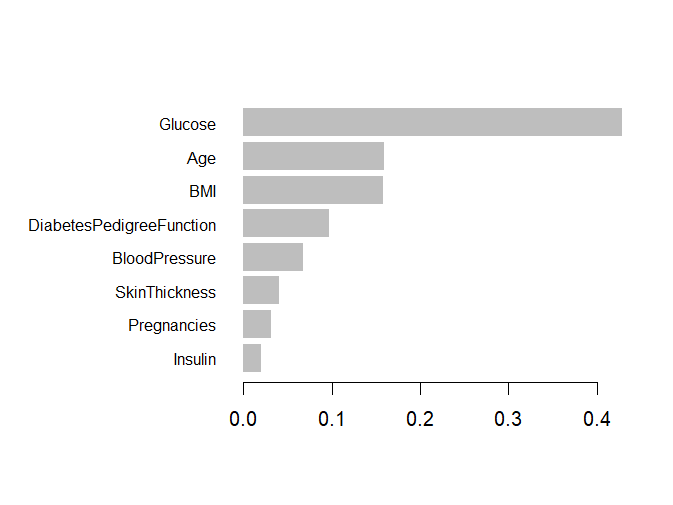
\includegraphics[width=\textwidth]{"C:/Users/msafi/OneDrive/Documents/GitHub/4m_final_project/G1.png"}}
		\caption{ROC Curve for Boosting Model}
		\label{fig:roc}
	\end{minipage}
	\hfill % Horizontal space between figures
	% Second figure
	\begin{minipage}{0.47\textwidth}
		\centering
		\fbox{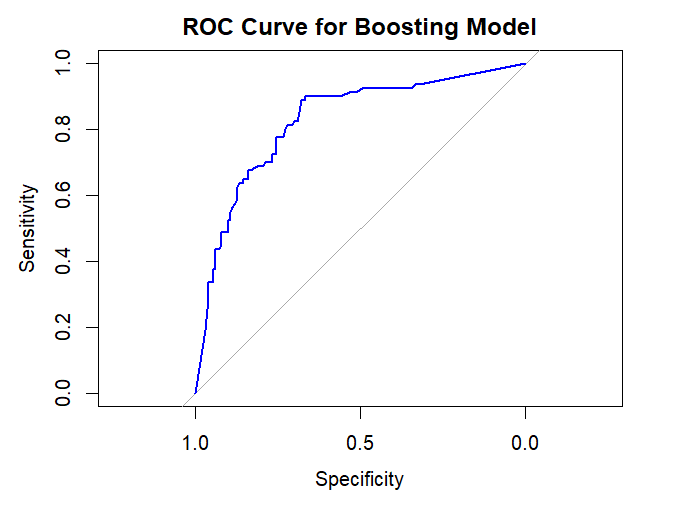
\includegraphics[width=\textwidth]{"C:/Users/msafi/OneDrive/Documents/GitHub/4m_final_project/G2.png"}}
		\caption{Feature Importance Plot}
		\label{fig:importance}
	\end{minipage}
\end{figure}


Boosting effectively identified significant predictors of diabetes, particularly glucose and BMI. However, the model's performance may be affected by missing data and the dataset's limited size. Future work could address these limitations by imputing missing values and validating the model on larger datasets. Overall, XGBoost proved to be a robust method for this binary classification problem.

\subsection{k-Nearest Neighbours}

% might want to include plot
After executing the tune.knn() function in $5$-fold cross validation. We found that the best value for $k$ is $5$. Then, after inputting $k=3$ into the knn() function, we found that the MCR of the k-nearest neighbours is $0.2916667$.

\subsection{Random Forest Classifiers}

%we wanna include the Variable importance plot here
After executing the tune.RandomForest() function in $5$-fold cross validation. We found that the best value for mtry is $4$ and the best value of ntree is $200$. Then, after inputting mtry $=4$ and ntree $=200$ into the RandomForest() function, we found that the MCR of the random forests is $0.28125$. \\
Finally, we also observe that Glucose and BMI are the two most important variables according to the variable importance plot.



\section{Conclusion}

\textbf{TEMPORARY, WILL IMPROVE LATER} Comparison between supervised and unsupervised learning analysis, which method performs better for this dataset, which version of machine learning analysis helps us draw better conclusions for our dataset etc. 

 \section{Bibliography}
 \bibliographystyle{apa} 
 \bibliography{references}

\end{document}

